\documentclass[a4paper,10pt]{article}
\usepackage[utf8]{inputenc}
\usepackage[T1]{fontenc}
\usepackage[provide=*,french]{babel}
\usepackage{lmodern}
\usepackage[left=0.72cm,right=0.72cm,top=0.48cm,bottom=0.78cm]{geometry}
\usepackage{tikz}
\usepackage{graphicx}
\usepackage{xcolor}
\usepackage{eso-pic}
\usepackage{amsmath,amssymb}
\usetikzlibrary{calc,arrows.meta,positioning}

\pagestyle{empty}
\renewcommand{\familydefault}{\sfdefault}
\setlength{\parindent}{0pt}

% Couleurs maths&go reprises de la fiche actuelle
\definecolor{brandNavy}{RGB}{11,53,112}
\definecolor{brandBlue}{RGB}{17,70,140}
\definecolor{brandSky}{RGB}{72,166,220}
\definecolor{brandTeal}{RGB}{29,174,174}
\definecolor{brandOrange}{RGB}{255,145,20}
\definecolor{softBlue}{RGB}{225,238,255}
\definecolor{softTeal}{RGB}{219,247,246}
\definecolor{softOrange}{RGB}{255,238,215}
\definecolor{softGray}{RGB}{245,247,250}
\definecolor{lightLine}{RGB}{190,230,230}

\newcommand{\LogoFile}{../assets/img/mathsgo-logo.png}
\newcommand{\MathsGoFooter}{%
\begin{tikzpicture}[remember picture,overlay]
  \node[anchor=south west,inner sep=0pt] at ([xshift=0.55cm,yshift=0.18cm]current page.south west)
    {\includegraphics[width=2.45cm]{\LogoFile}};
  \node[anchor=south,inner sep=0pt,text=brandNavy!70,font=\sffamily\bfseries\fontsize{7}{7}\selectfont]
    at ([yshift=0.32cm]current page.south) {mathsgo.re \textperiodcentered\ CC BY-NC-SA 4.0};
\end{tikzpicture}%
}
\AddToShipoutPictureFG{\MathsGoFooter}

\newcommand{\Badge}[1]{\tikz[baseline=-0.62ex]{\node[circle,fill=brandNavy,text=white,font=\bfseries,minimum size=0.50cm,inner sep=0pt]{#1};}}
\newcommand{\Section}[2]{\Badge{#1}\hspace{0.15cm}{\bfseries\color{brandNavy}\fontsize{11.7}{12.4}\selectfont #2}}
\newcommand{\Apt}{\textcolor{brandOrange}{A}}
\newcommand{\Mpt}{\textcolor{brandBlue}{M}}
\newcommand{\Npt}{\textcolor{brandBlue}{N}}
\newcommand{\Bpt}{\textcolor{brandTeal}{B}}
\newcommand{\Cpt}{\textcolor{brandTeal}{C}}
\newcommand{\AMcol}{\textcolor{brandOrange}{A}\textcolor{brandBlue}{M}}
\newcommand{\ANcol}{\textcolor{brandOrange}{A}\textcolor{brandBlue}{N}}
\newcommand{\ABcol}{\textcolor{brandOrange}{A}\textcolor{brandTeal}{B}}
\newcommand{\ACcol}{\textcolor{brandOrange}{A}\textcolor{brandTeal}{C}}
\newcommand{\MNcol}{\textcolor{brandBlue}{M}\textcolor{brandBlue}{N}}
\newcommand{\BCcol}{\textcolor{brandTeal}{B}\textcolor{brandTeal}{C}}

% Figures reprises de la fiche actuelle
\newcommand{\FigureEmboitee}[1]{%
\begin{tikzpicture}[scale=#1,line cap=butt,line join=miter]
  \coordinate (A) at (0,0);
  \coordinate (B) at (5.40,-1.20);
  \coordinate (C) at (4.70,2.20);
  \coordinate (M) at (2.59,-0.58);
  \coordinate (N) at (2.26,1.06);
  \fill[softTeal!38] (A)--(B)--(C)--cycle;
  % Le grand triangle reste visible sous le petit : halo leger, puis trait reel
  % de meme epaisseur que les cotes bleu fonce places au premier plan.
  \draw[brandSky!65,line width=2.30pt] (A)--(B);
  \draw[brandSky!65,line width=2.30pt] (A)--(C);
  \draw[brandSky,line width=1.20pt] (A)--(B);
  \draw[brandSky,line width=1.20pt] (A)--(C);
  \draw[brandNavy,line width=1.20pt] (A)--(M);
  \draw[brandNavy,line width=1.20pt] (A)--(N);
  \draw[brandNavy,line width=1.24pt] (M)--(N);
  \draw[brandTeal,line width=1.34pt] (B)--(C);
  \node[brandOrange,font=\bfseries\small] at (-0.27,-0.25) {$A$};
  \node[brandBlue,font=\bfseries\small] at (2.62,-0.88) {$M$};
  \node[brandBlue,font=\bfseries\small] at (2.04,1.28) {$N$};
  \node[brandTeal,font=\bfseries\small] at (5.68,-1.18) {$B$};
  \node[brandTeal,font=\bfseries\small] at (4.89,2.42) {$C$};
\end{tikzpicture}}

\newcommand{\FigurePapillon}[1]{%
\begin{tikzpicture}[scale=#1,line cap=butt,line join=miter]
  \coordinate (A) at (0,0);
  \coordinate (B) at (3.40,-1.20);
  \coordinate (C) at (2.60,1.90);
  \coordinate (M) at (-2.21,0.78);
  \coordinate (N) at (-1.69,-1.24);
  \draw[brandNavy,line width=1.20pt] (M)--(A);
  \draw[brandNavy,line width=1.20pt] (N)--(A);
  \draw[brandNavy,line width=1.24pt] (M)--(N);
  \draw[brandTeal,line width=1.20pt] (A)--(B);
  \draw[brandTeal,line width=1.20pt] (A)--(C);
  \draw[brandTeal,line width=1.34pt] (B)--(C);
  \node[brandOrange,font=\bfseries\small] at (-0.05,0.31) {$A$};
  \node[brandBlue,font=\bfseries\small] at (-2.50,0.94) {$M$};
  \node[brandBlue,font=\bfseries\small] at (-1.93,-1.43) {$N$};
  \node[brandTeal,font=\bfseries\small] at (3.68,-1.21) {$B$};
  \node[brandTeal,font=\bfseries\small] at (2.80,2.12) {$C$};
\end{tikzpicture}}

\newcommand{\OrderLine}[3]{%
  \tikz[baseline=-0.65ex]{\node[rounded corners=4pt,fill=#1!9,draw=#1!55,line width=.55pt,text width=7.85cm,inner xsep=6pt,inner ysep=3pt,align=left]
  {\bfseries\fontsize{8.8}{9.4}\selectfont #2\hfill\textcolor{brandNavy}{#3}};}}
\newcommand{\LowDotted}[1]{%
\begin{tikzpicture}[baseline=-0.78ex]
  \draw[densely dotted,line width=0.70pt,line cap=round] (0,-0.22) -- (#1,-0.22);
\end{tikzpicture}}
\newcommand{\CheckBox}{\ensuremath{\Box}\,}
\newcommand{\BigRatio}[1]{{\fontsize{15.0}{16.0}\selectfont\displaystyle #1}}

\newcommand{\BlankEmboitee}[1]{%
\begin{tikzpicture}[scale=#1,line cap=butt,line join=miter]
  \coordinate (A) at (0,0);
  \coordinate (B) at (5.40,-1.20);
  \coordinate (C) at (4.70,2.20);
  \coordinate (M) at (2.59,-0.58);
  \coordinate (N) at (2.26,1.06);
  \fill[softTeal!22] (A)--(B)--(C)--cycle;
  \draw[brandSky!65,line width=2.20pt] (A)--(B);
  \draw[brandSky!65,line width=2.20pt] (A)--(C);
  \draw[brandSky,line width=1.10pt] (A)--(B);
  \draw[brandSky,line width=1.10pt] (A)--(C);
  \draw[brandNavy!90,line width=1.10pt] (A)--(M);
  \draw[brandNavy!90,line width=1.10pt] (A)--(N);
  \draw[brandNavy!90,line width=1.15pt] (M)--(N);
  \draw[brandTeal,line width=1.18pt] (B)--(C);
  \node at (-0.55,-0.45) {\LowDotted{0.48}};
  \node at (2.82,-1.08) {\LowDotted{0.48}};
  \node at (1.82,1.50) {\LowDotted{0.48}};
  \node at (6.02,-1.35) {\LowDotted{0.48}};
  \node at (4.90,2.68) {\LowDotted{0.48}};
\end{tikzpicture}}

\newcommand{\BlankPapillon}[1]{%
\begin{tikzpicture}[scale=#1,line cap=butt,line join=miter]
  \coordinate (A) at (0,0);
  \coordinate (B) at (3.40,-1.20);
  \coordinate (C) at (2.60,1.90);
  \coordinate (M) at (-2.21,0.78);
  \coordinate (N) at (-1.69,-1.24);
  \draw[brandNavy!90,line width=1.10pt] (M)--(A);
  \draw[brandNavy!90,line width=1.10pt] (N)--(A);
  \draw[brandNavy!90,line width=1.15pt] (M)--(N);
  \draw[brandTeal,line width=1.10pt] (A)--(B);
  \draw[brandTeal,line width=1.10pt] (A)--(C);
  \draw[brandTeal,line width=1.18pt] (B)--(C);
  \node at (0.00,0.55) {\LowDotted{0.48}};
  \node at (-2.72,1.20) {\LowDotted{0.48}};
  \node at (-2.05,-1.68) {\LowDotted{0.48}};
  \node at (4.00,-1.40) {\LowDotted{0.48}};
  \node at (2.95,2.38) {\LowDotted{0.48}};
\end{tikzpicture}}

\begin{document}

\begin{center}
{\fontsize{21.0}{22.0}\selectfont\bfseries\color{brandNavy} Thalès : tester un parallélisme}\par\vspace{0.01cm}
{\fontsize{12.4}{13.1}\selectfont\bfseries\color{brandTeal} Réciproque ou contraposée ?}\par\vspace{0.01cm}
{\fontsize{8.8}{9.4}\selectfont\bfseries\color{brandOrange} Comprendre avant de rédiger}
\end{center}

\vspace{0.02cm}
\begin{center}
\begin{minipage}[t]{9.15cm}
\centering
\tikz\node[rounded corners=7pt,draw=brandTeal!65,fill=brandTeal!3,line width=0.70pt,text width=8.70cm,inner sep=5pt,align=center]{%
{\bfseries\color{brandTeal} Cas emboîté}\par\vspace{-0.02cm}
\FigureEmboitee{0.62}\par\vspace{-0.03cm}
{\small $\Apt-\Mpt-\Bpt$ \qquad et \qquad $\Apt-\Npt-\Cpt$}
};
\end{minipage}\hfill
\begin{minipage}[t]{9.15cm}
\centering
\tikz\node[rounded corners=7pt,draw=brandOrange!70,fill=softOrange!25,line width=0.70pt,text width=8.70cm,inner sep=5pt,align=center]{%
{\bfseries\color{brandOrange} Cas papillon}\par\vspace{-0.02cm}
\FigurePapillon{0.66}\par\vspace{-0.03cm}
{\small $\Mpt-\Apt-\Bpt$ \qquad et \qquad $\Npt-\Apt-\Cpt$}
};
\end{minipage}
\end{center}

\vspace{0.14cm}
\Section{1}{Je vérifie le contexte}\par\vspace{0.05cm}
\begin{center}

\begin{tikzpicture}
\node[rounded corners=7pt,draw=brandNavy!42,fill=softBlue!26,line width=.70pt,text width=17.75cm,inner sep=5.5pt,align=center] {
{\fontsize{9.2}{9.9}\selectfont Les points $A,M,B$ sont alignés. Les points $A,N,C$ sont alignés. $A$ est le sommet commun. Les droites à tester sont $(MN)$ et $(BC)$.}
};
\end{tikzpicture}
\end{center}

\vspace{0.10cm}
\Section{2}{Je construis les deux rapports à comparer}\par\vspace{0.06cm}
\begin{center}

\begin{tikzpicture}
\node[rounded corners=7pt,draw=brandNavy!42,fill=softBlue!26,line width=.70pt,text width=17.75cm,inner sep=8pt,align=center] {
{\fontsize{9.5}{10.2}\selectfont Sur chaque droite, je pars de \Apt{} et je garde \textbf{le même ordre} : longueur jusqu'au premier point, puis longueur jusqu'au second point.}\par\vspace{0.05cm}
{\fontsize{16}{17}\selectfont $\displaystyle \frac{\AMcol}{\ABcol}$}\hspace{0.85cm}{\bfseries\color{brandNavy} et}\hspace{0.85cm}{\fontsize{16}{17}\selectfont $\displaystyle \frac{\ANcol}{\ACcol}$}
\par\vspace{0.02cm}
{\fontsize{8.5}{9.1}\selectfont\bfseries\color{brandOrange} Je ne dis pas encore que les rapports sont égaux : je vais d'abord les calculer.}
};
\end{tikzpicture}
\end{center}

\vspace{0.17cm}
\Section{3}{Je calcule les deux rapports, puis je les compare}\par\vspace{0.06cm}
\noindent\begin{minipage}[t]{9.15cm}
\vspace{0pt}
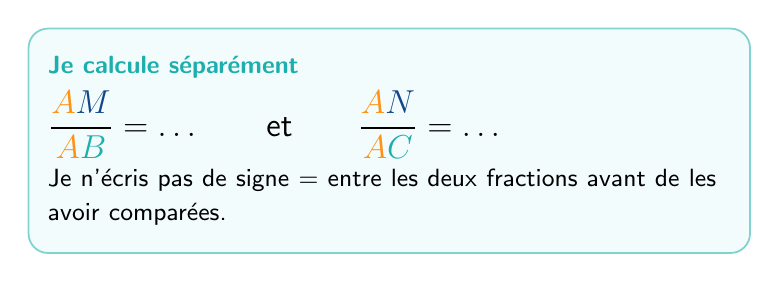
\begin{tikzpicture}
\node[rounded corners=7pt,draw=brandTeal!55,fill=softTeal!35,line width=.65pt,text width=8.67cm,minimum height=2.85cm,inner sep=7pt,align=left] {
{\bfseries\color{brandTeal}\fontsize{9.3}{10.0}\selectfont Je calcule séparément}\par\vspace{0.12cm}
{\fontsize{12.8}{13.6}\selectfont $\displaystyle \frac{\AMcol}{\ABcol}=\ldots \qquad\text{et}\qquad \frac{\ANcol}{\ACcol}=\ldots$}\par\vspace{0.10cm}
{\fontsize{8.8}{9.5}\selectfont Je n'écris pas de signe $=$ entre les deux fractions avant de les avoir comparées.}
};
\end{tikzpicture}
\end{minipage}\hfill
\begin{minipage}[t]{9.15cm}
\vspace{0pt}
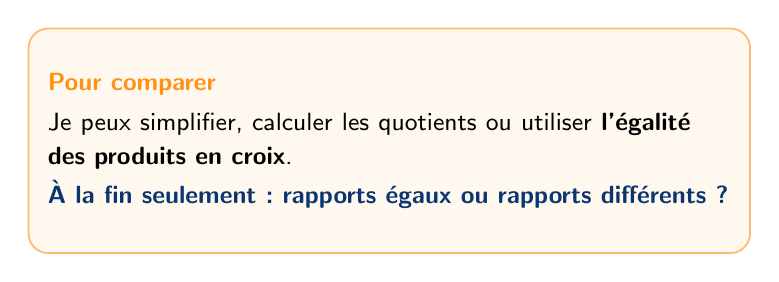
\begin{tikzpicture}
\node[rounded corners=7pt,draw=brandOrange!62,fill=softOrange!42,line width=.65pt,text width=8.67cm,minimum height=2.85cm,inner sep=7pt,align=left] {
{\bfseries\color{brandOrange}\fontsize{9.3}{10.0}\selectfont Pour comparer}\par\vspace{0.09cm}
{\fontsize{9.0}{9.7}\selectfont Je peux simplifier, calculer les quotients ou utiliser \textbf{l'égalité des produits en croix}.}\par\vspace{0.08cm}
{\fontsize{8.8}{9.5}\selectfont\bfseries\color{brandNavy} À la fin seulement : rapports égaux ou rapports différents ?}
};
\end{tikzpicture}
\end{minipage}

\vspace{0.17cm}
\Section{4}{J'observe le résultat, puis j'applique le bon critère}\par\vspace{0.06cm}
\begin{center}
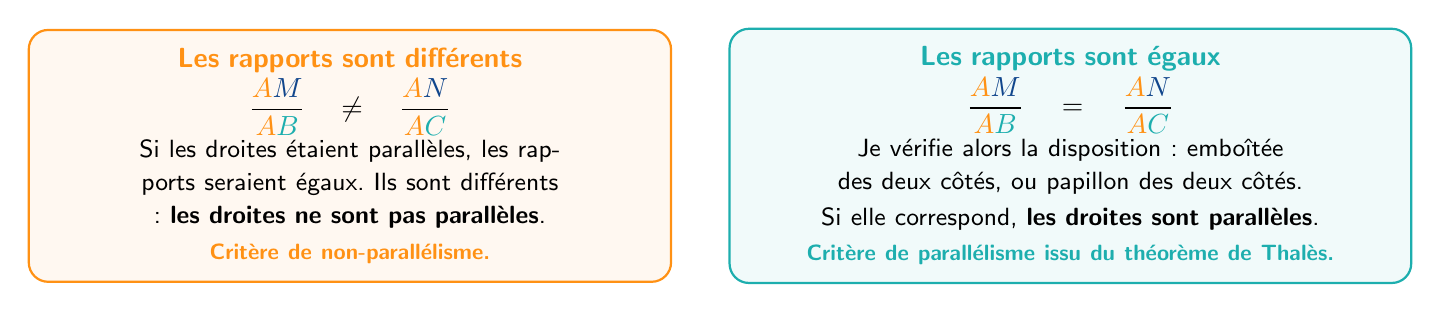
\begin{tikzpicture}
\node[rounded corners=7pt,draw=brandOrange,fill=brandOrange!6,line width=.80pt,text width=7.70cm,minimum height=3.15cm,inner sep=6.5pt,align=center] (diff) at (-4.70,-1.55)
{{\bfseries\color{brandOrange}\fontsize{10.1}{10.8}\selectfont Les rapports sont différents}\par\vspace{0.04cm}
$\displaystyle \frac{\AMcol}{\ABcol}\neq\frac{\ANcol}{\ACcol}$\par\vspace{0.03cm}
{\fontsize{9.0}{9.6}\selectfont Si les droites étaient parallèles, les rapports seraient égaux. Ils sont différents : \textbf{les droites ne sont pas parallèles}.}\par\vspace{0.03cm}
{\fontsize{8.2}{8.8}\selectfont\bfseries\color{brandOrange} Critère de non-parallélisme.}};

\node[rounded corners=7pt,draw=brandTeal,fill=brandTeal!6,line width=.80pt,text width=8.20cm,minimum height=3.15cm,inner sep=6.5pt,align=center] (equal) at (4.45,-1.55)
{{\bfseries\color{brandTeal}\fontsize{10.1}{10.8}\selectfont Les rapports sont égaux}\par\vspace{0.04cm}
$\displaystyle \frac{\AMcol}{\ABcol}=\frac{\ANcol}{\ACcol}$\par\vspace{0.03cm}
{\fontsize{8.9}{9.5}\selectfont Je vérifie alors la disposition : emboîtée des deux côtés, ou papillon des deux côtés.}\par\vspace{0.03cm}
{\fontsize{8.9}{9.5}\selectfont Si elle correspond, \textbf{les droites sont parallèles}.}\par\vspace{0.03cm}
{\fontsize{8.2}{8.8}\selectfont\bfseries\color{brandTeal} Critère de parallélisme issu du théorème de Thalès.}};

\end{tikzpicture}
\end{center}

\vspace{0.17cm}
\Section{5}{Deux rédactions qui expliquent le raisonnement}\par\vspace{0.06cm}
\noindent\begin{minipage}[t]{9.15cm}
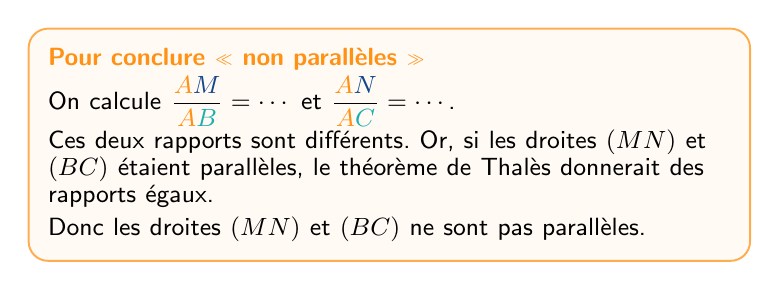
\begin{tikzpicture}
\node[rounded corners=7pt,draw=brandOrange!75,fill=softOrange!28,line width=.70pt,text width=8.67cm,minimum height=2.75cm,inner sep=7pt,align=left] {
{\bfseries\color{brandOrange}\fontsize{9.4}{10.0}\selectfont Pour conclure « non parallèles »}\par\vspace{0.05cm}
{\fontsize{9.0}{9.7}\selectfont
On calcule $\dfrac{\AMcol}{\ABcol}=\cdots$ et $\dfrac{\ANcol}{\ACcol}=\cdots$.\par
Ces deux rapports sont différents. Or, si les droites $(MN)$ et $(BC)$ étaient parallèles, le théorème de Thalès donnerait des rapports égaux.\par
Donc les droites $(MN)$ et $(BC)$ ne sont pas parallèles.}
};
\end{tikzpicture}
\end{minipage}\hfill
\begin{minipage}[t]{9.15cm}
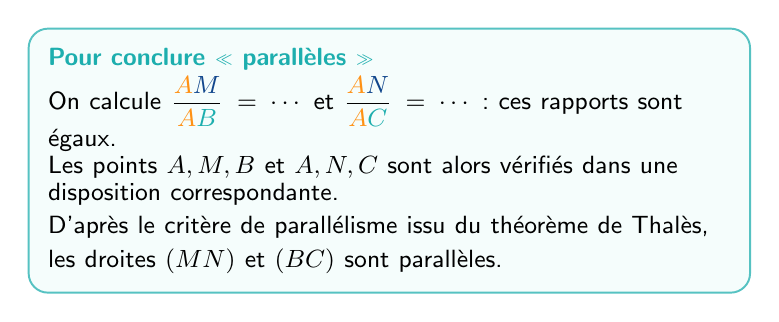
\begin{tikzpicture}
\node[rounded corners=7pt,draw=brandTeal!75,fill=softTeal!28,line width=.70pt,text width=8.67cm,minimum height=2.75cm,inner sep=7pt,align=left] {
{\bfseries\color{brandTeal}\fontsize{9.4}{10.0}\selectfont Pour conclure « parallèles »}\par\vspace{0.05cm}
{\fontsize{9.0}{9.7}\selectfont
On calcule $\dfrac{\AMcol}{\ABcol}=\cdots$ et $\dfrac{\ANcol}{\ACcol}=\cdots$ : ces rapports sont égaux.\par
Les points $A,M,B$ et $A,N,C$ sont alors vérifiés dans une disposition correspondante.\par
D'après le critère de parallélisme issu du théorème de Thalès, les droites $(MN)$ et $(BC)$ sont parallèles.}
};
\end{tikzpicture}
\end{minipage}

\newpage

\begin{center}
{\fontsize{20.0}{21.0}\selectfont\bfseries\color{brandNavy} Fiche-guide : tester un parallélisme}\par\vspace{0.02cm}
{\fontsize{11.8}{12.5}\selectfont\bfseries\color{brandTeal} J'adapte les lettres à la figure de mon exercice}
\end{center}

\vspace{0.10cm}
\noindent
\begin{minipage}[t]{5.20cm}
\vspace{0pt}
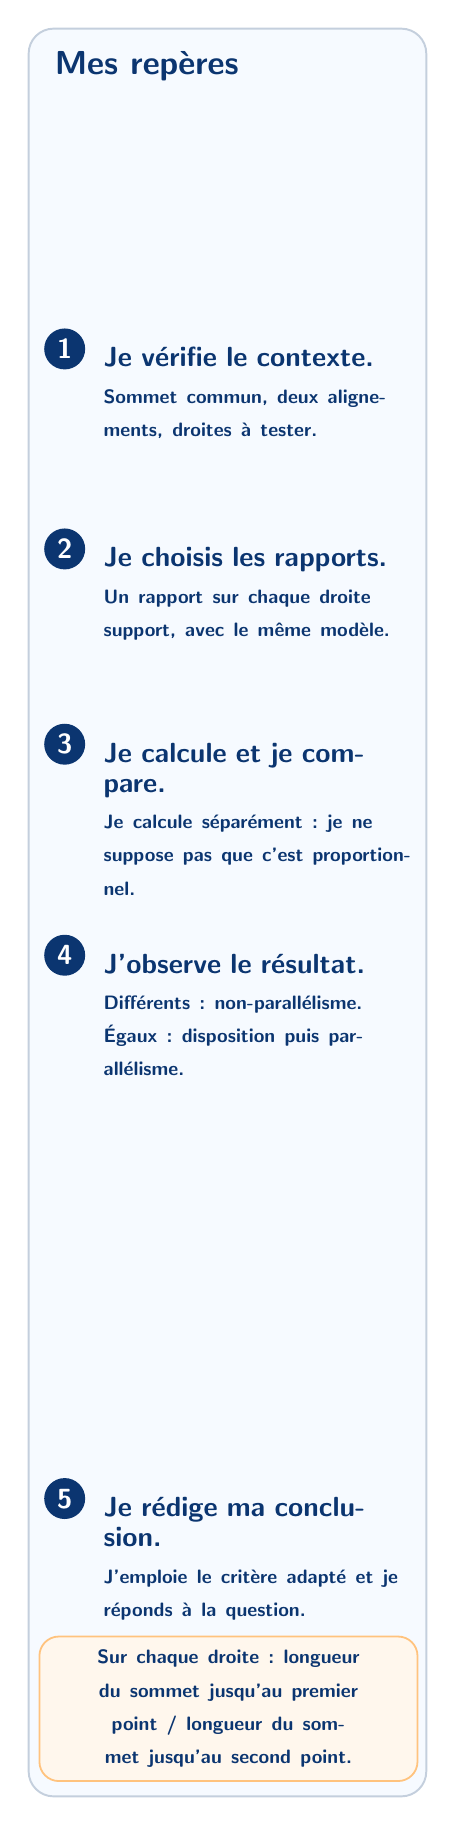
\begin{tikzpicture}[x=1cm,y=1cm]
\path[use as bounding box] (0,0) rectangle (5.20,-22.70);
\node[rounded corners=9pt,draw=brandNavy!24,fill=softBlue!30,line width=0.70pt,minimum width=5.05cm,minimum height=22.45cm,anchor=north west] at (0,0) {};
\node[anchor=north west,text=brandNavy,font=\bfseries\fontsize{12.0}{12.8}\selectfont] at (0.22,-0.18) {Mes repères};

\node[circle,fill=brandNavy,text=white,font=\bfseries,minimum size=0.52cm,inner sep=0pt] at (0.47,-4.08) {1};
\node[anchor=north west,text width=3.92cm,align=left] at (0.84,-3.94) {\bfseries\color{brandNavy}\fontsize{10.2}{10.9}\selectfont Je vérifie le contexte.\par\vspace{0.04cm}
{\scriptsize\bfseries\color{brandNavy} Sommet commun, deux alignements, droites à tester.}};

\node[circle,fill=brandNavy,text=white,font=\bfseries,minimum size=0.52cm,inner sep=0pt] at (0.47,-6.62) {2};
\node[anchor=north west,text width=3.92cm,align=left] at (0.84,-6.48) {\bfseries\color{brandNavy}\fontsize{10.2}{10.9}\selectfont Je choisis les rapports.\par\vspace{0.04cm}
{\scriptsize\bfseries\color{brandNavy} Un rapport sur chaque droite support, avec le même modèle.}};

\node[circle,fill=brandNavy,text=white,font=\bfseries,minimum size=0.52cm,inner sep=0pt] at (0.47,-9.10) {3};
\node[anchor=north west,text width=3.92cm,align=left] at (0.84,-8.96) {\bfseries\color{brandNavy}\fontsize{10.2}{10.9}\selectfont Je calcule et je compare.\par\vspace{0.04cm}
{\scriptsize\bfseries\color{brandNavy} Je calcule séparément : je ne suppose pas que c'est proportionnel.}};

\node[circle,fill=brandNavy,text=white,font=\bfseries,minimum size=0.52cm,inner sep=0pt] at (0.47,-11.78) {4};
\node[anchor=north west,text width=3.92cm,align=left] at (0.84,-11.64) {\bfseries\color{brandNavy}\fontsize{10.2}{10.9}\selectfont J'observe le résultat.\par\vspace{0.04cm}
{\scriptsize\bfseries\color{brandNavy} Différents : non-parallélisme. Égaux : disposition puis parallélisme.}};

\node[circle,fill=brandNavy,text=white,font=\bfseries,minimum size=0.52cm,inner sep=0pt] at (0.47,-18.68) {5};
\node[anchor=north west,text width=3.92cm,align=left] at (0.84,-18.54) {\bfseries\color{brandNavy}\fontsize{10.2}{10.9}\selectfont Je rédige ma conclusion.\par\vspace{0.04cm}
{\scriptsize\bfseries\color{brandNavy} J'emploie le critère adapté et je réponds à la question.}};

\node[rounded corners=7pt,draw=brandOrange!55,fill=softOrange!45,line width=0.65pt,text width=4.45cm,inner sep=5pt,align=center] at (2.55,-21.35) {\scriptsize\bfseries\color{brandNavy} Sur chaque droite : longueur du sommet jusqu'au premier point / longueur du sommet jusqu'au second point.};
\end{tikzpicture}
\end{minipage}\hfill
\begin{minipage}[t]{13.20cm}
\vspace{0pt}

{\bfseries\color{brandTeal}\fontsize{10.8}{11.4}\selectfont J'entoure le cas et je place les lettres de l'exercice.}\par\vspace{0.04cm}
\begin{center}
\begin{minipage}[t]{6.25cm}
\centering
\tikz\node[rounded corners=8pt,draw=brandTeal!65,fill=brandTeal!3,line width=0.75pt,text width=5.80cm,inner sep=5pt,align=center]{%
{\bfseries\color{brandTeal}\CheckBox cas emboîté}\par\vspace{0.02cm}
\BlankEmboitee{0.49}
};
\end{minipage}\hfill
\begin{minipage}[t]{6.25cm}
\centering
\tikz\node[rounded corners=8pt,draw=brandOrange!70,fill=softOrange!25,line width=0.75pt,text width=5.80cm,inner sep=5pt,align=center]{%
{\bfseries\color{brandOrange}\CheckBox cas papillon}\par\vspace{0.02cm}
\BlankPapillon{0.54}
};
\end{minipage}
\end{center}

\vspace{0.20cm}
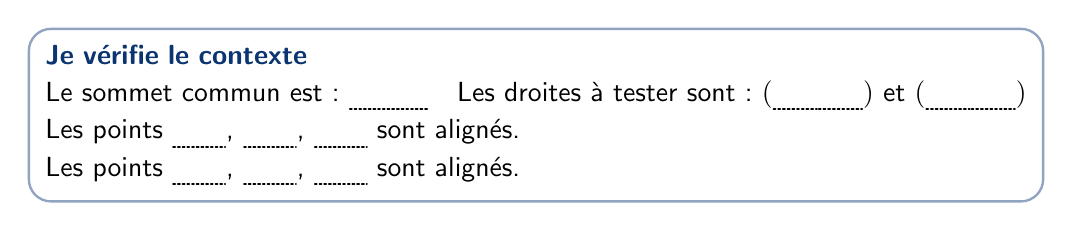
\begin{tikzpicture}
\node[rounded corners=8pt,draw=brandNavy!45,fill=white,line width=0.85pt,text width=12.46cm,inner sep=6.0pt,align=left] {
{\bfseries\color{brandNavy}\fontsize{9.9}{11.1}\selectfont Je vérifie le contexte}\par\vspace{0.04cm}
{\fontsize{9.9}{11.1}\selectfont Le sommet commun est : \LowDotted{1.00}\hfill Les droites à tester sont : $(\LowDotted{0.55}\LowDotted{0.55})$ et $(\LowDotted{0.55}\LowDotted{0.55})$}\par\vspace{0.06cm}
{\fontsize{9.9}{11.1}\selectfont Les points \LowDotted{0.66}, \LowDotted{0.66}, \LowDotted{0.66} sont alignés.}\par\vspace{0.05cm}
{\fontsize{9.9}{11.1}\selectfont Les points \LowDotted{0.66}, \LowDotted{0.66}, \LowDotted{0.66} sont alignés.}
};
\end{tikzpicture}

\vspace{0.24cm}
{\bfseries\color{brandNavy}\fontsize{11.4}{12.2}\selectfont Je choisis les deux rapports}\par\vspace{0.04cm}
\begin{center}
$\begin{array}{rcl}
\BigRatio{\dfrac{\LowDotted{0.80}}{\LowDotted{0.80}}} & = & \BigRatio{\dfrac{\LowDotted{0.74}}{\LowDotted{0.74}}=\LowDotted{0.86}}\\[0.30cm]
\BigRatio{\dfrac{\LowDotted{0.80}}{\LowDotted{0.80}}} & = & \BigRatio{\dfrac{\LowDotted{0.74}}{\LowDotted{0.74}}=\LowDotted{0.86}}
\end{array}$
\end{center}

\vspace{0.06cm}
{\bfseries\color{brandNavy}\fontsize{11.0}{11.8}\selectfont Je les calcule et je les compare}\par\vspace{0.10cm}

\begin{tikzpicture}
\node[rounded corners=7pt,draw=brandOrange!55,fill=softOrange!38,line width=0.65pt,text width=12.46cm,inner sep=4.8pt,align=center] {\bfseries\color{brandNavy} Pour comparer : je simplifie, je calcule les quotients, ou j'utilise l'égalité des produits en croix.};
\end{tikzpicture}

\vspace{0.20cm}
{\bfseries\color{brandNavy}\fontsize{11.0}{11.8}\selectfont J'observe le résultat}\par\vspace{0.08cm}
\noindent\begin{minipage}[t]{6.30cm}
\vspace{0pt}
{\bfseries\color{brandOrange}\fontsize{10.1}{10.8}\selectfont \CheckBox Les rapports sont différents}\par\vspace{0.04cm}
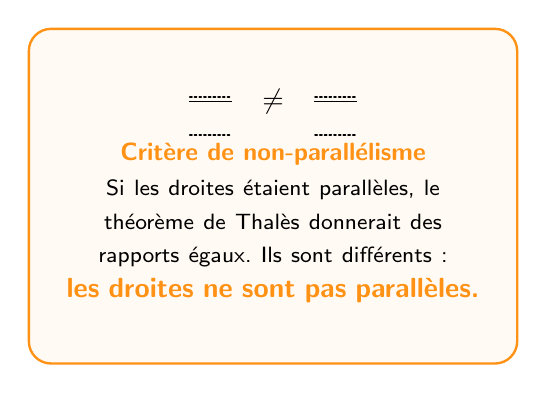
\begin{tikzpicture}
\node[rounded corners=8pt,draw=brandOrange,fill=brandOrange!5,line width=0.85pt,text width=5.78cm,minimum height=4.25cm,inner sep=6.0pt,align=center] {
$\displaystyle \frac{\LowDotted{0.52}}{\LowDotted{0.52}}\neq\frac{\LowDotted{0.52}}{\LowDotted{0.52}}$\par\vspace{0.05cm}
{\fontsize{8.9}{9.5}\selectfont\bfseries\color{brandOrange} Critère de non-parallélisme}\par\vspace{0.03cm}
{\fontsize{8.3}{8.9}\selectfont Si les droites étaient parallèles, le théorème de Thalès donnerait des rapports égaux. Ils sont différents :}\par\vspace{0.03cm}
{\bfseries\color{brandOrange} les droites ne sont pas parallèles.}
};
\end{tikzpicture}
\end{minipage}\hfill
\begin{minipage}[t]{6.30cm}
\vspace{0pt}
{\bfseries\color{brandTeal}\fontsize{10.1}{10.8}\selectfont \CheckBox Les rapports sont égaux}\par\vspace{0.04cm}
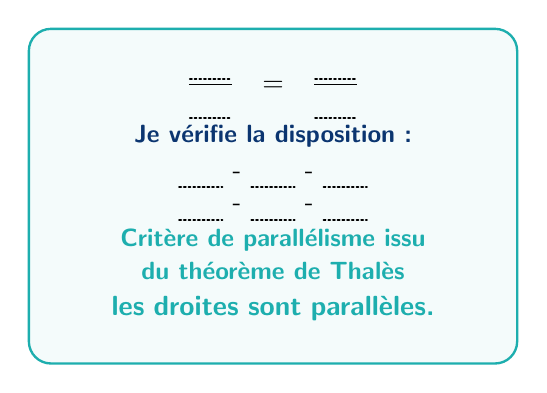
\begin{tikzpicture}
\node[rounded corners=8pt,draw=brandTeal,fill=brandTeal!5,line width=0.85pt,text width=5.78cm,minimum height=4.25cm,inner sep=6.0pt,align=center] {
$\displaystyle \frac{\LowDotted{0.52}}{\LowDotted{0.52}}=\frac{\LowDotted{0.52}}{\LowDotted{0.52}}$\par\vspace{0.05cm}
{\fontsize{8.9}{9.5}\selectfont\bfseries\color{brandNavy} Je vérifie la disposition :}\par\vspace{0.03cm}
{\small \LowDotted{0.55} - \LowDotted{0.55} - \LowDotted{0.55}}\par\vspace{-0.01cm}
{\small \LowDotted{0.55} - \LowDotted{0.55} - \LowDotted{0.55}}\par\vspace{0.03cm}
{\fontsize{8.8}{9.4}\selectfont\bfseries\color{brandTeal} Critère de parallélisme issu du théorème de Thalès}\par\vspace{0.03cm}
{\bfseries\color{brandTeal} les droites sont parallèles.}
};
\end{tikzpicture}
\end{minipage}

\vspace{0.24cm}
{\bfseries\color{brandNavy}\fontsize{11.0}{11.8}\selectfont Je rédige ma conclusion}\par\vspace{0.05cm}
\begin{center}
\tikz[baseline=-0.72ex]{\node[rounded corners=6pt,draw=brandNavy!55,fill=softBlue!18,line width=0.8pt,inner xsep=12pt,inner ysep=6.2pt,font=\bfseries\fontsize{11.0}{11.7}\selectfont\color{brandNavy}]{Donc les droites $(\LowDotted{0.62}\LowDotted{0.62})$ et $(\LowDotted{0.62}\LowDotted{0.62})$ sont \LowDotted{2.35}.};}
\end{center}

\vspace{0.26cm}
\begin{center}

\begin{tikzpicture}
\node[rounded corners=7pt,draw=brandOrange!55,fill=softOrange!50,line width=0.65pt,text width=12.46cm,inner sep=5.0pt,align=center] {\bfseries\color{brandNavy} J'ai appliqué le critère de : \hspace{0.20cm}$\Box$ parallélisme \hspace{0.16cm}$\Box$ non-parallélisme};
\end{tikzpicture}
\end{center}

\end{minipage}

\newpage

\begin{center}
{\fontsize{20.0}{21.0}\selectfont\bfseries\color{brandNavy} Deux exemples entièrement rédigés}\par\vspace{0.02cm}
{\fontsize{11.8}{12.5}\selectfont\bfseries\color{brandTeal} Un cas emboîté et un cas papillon}
\end{center}

\vspace{0.28cm}
{\bfseries\color{brandTeal}\fontsize{12.5}{13.3}\selectfont Exemple 1 — je peux conclure « parallèles »}\par\vspace{0.05cm}
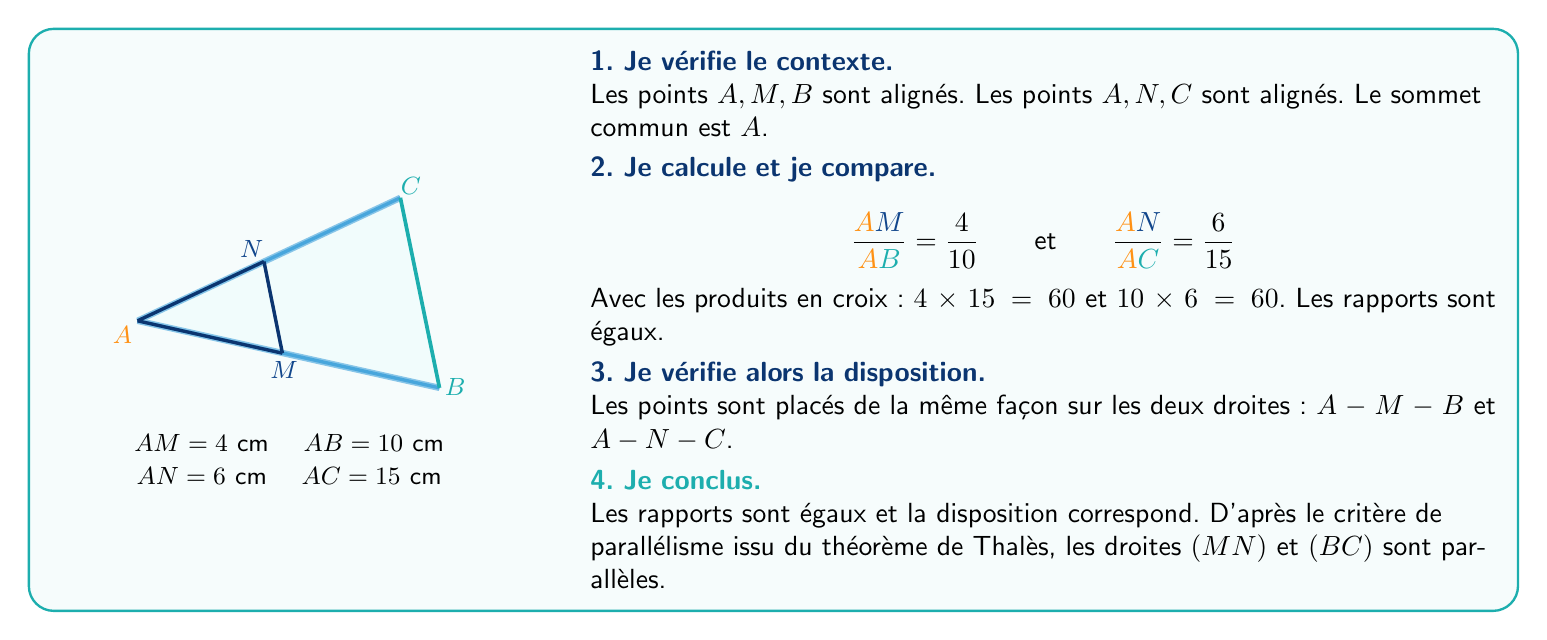
\begin{tikzpicture}
\node[rounded corners=9pt,draw=brandTeal,fill=brandTeal!4,line width=.85pt,text width=18.35cm,inner sep=8pt,align=left] {
\begin{minipage}[c]{6.05cm}
\centering
\FigureEmboitee{0.71}\par\vspace{0.08cm}
{\fontsize{9.4}{10.1}\selectfont $AM=4$ cm \quad $AB=10$ cm\par $AN=6$ cm \quad $AC=15$ cm}
\end{minipage}\hfill
\begin{minipage}[c]{11.50cm}
{\bfseries\color{brandNavy} 1. Je vérifie le contexte.}\par
Les points $A,M,B$ sont alignés. Les points $A,N,C$ sont alignés. Le sommet commun est $A$.\par\vspace{0.08cm}
{\bfseries\color{brandNavy} 2. Je calcule et je compare.}\par
\[
\frac{\AMcol}{\ABcol}=\frac{4}{10}
\qquad\text{et}\qquad
\frac{\ANcol}{\ACcol}=\frac{6}{15}
\]
Avec les produits en croix : $4\times15=60$ et $10\times6=60$. Les rapports sont égaux.\par\vspace{0.10cm}
{\bfseries\color{brandNavy} 3. Je vérifie alors la disposition.}\par
Les points sont placés de la même façon sur les deux droites : $A-M-B$ et $A-N-C$.\par\vspace{0.10cm}
{\bfseries\color{brandTeal} 4. Je conclus.}\par
Les rapports sont égaux et la disposition correspond. D'après le critère de parallélisme issu du théorème de Thalès, les droites $(MN)$ et $(BC)$ sont parallèles.
\end{minipage}
};
\end{tikzpicture}

\vspace{0.56cm}
{\bfseries\color{brandOrange}\fontsize{12.5}{13.3}\selectfont Exemple 2 — je conclus « non parallèles »}\par\vspace{0.05cm}
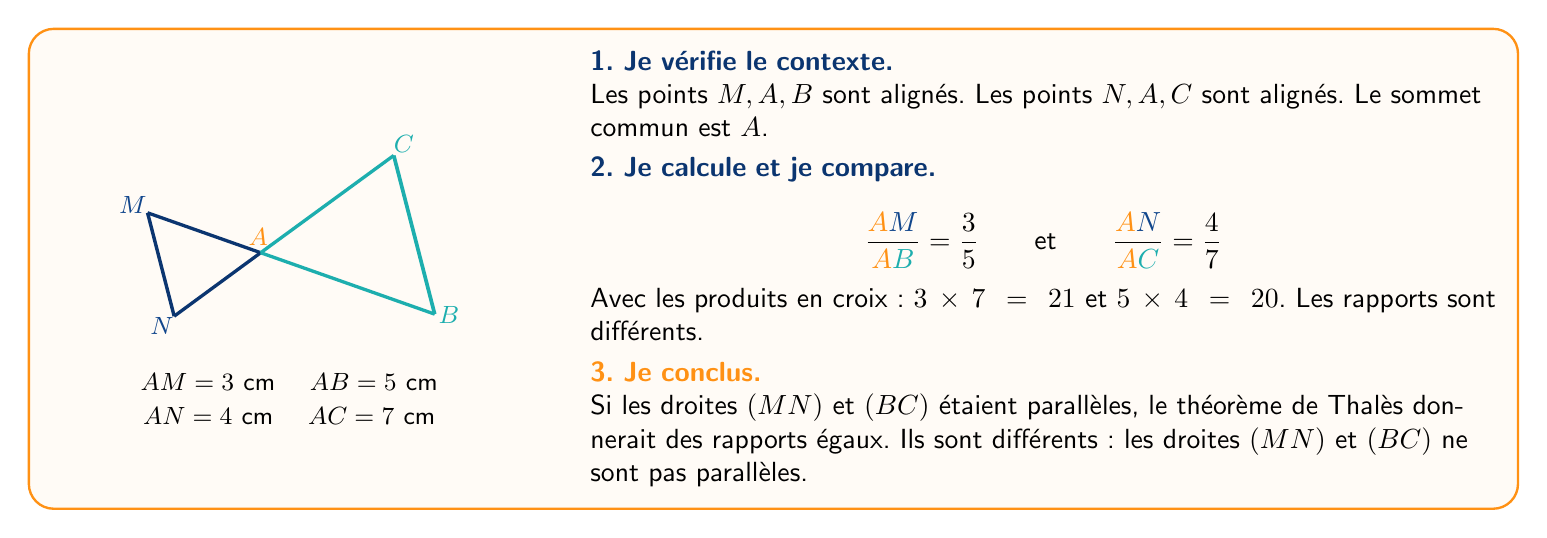
\begin{tikzpicture}
\node[rounded corners=9pt,draw=brandOrange,fill=brandOrange!4,line width=.85pt,text width=18.35cm,inner sep=8pt,align=left] {
\begin{minipage}[c]{6.05cm}
\centering
\FigurePapillon{0.65}\par\vspace{0.08cm}
{\fontsize{9.4}{10.1}\selectfont $AM=3$ cm \quad $AB=5$ cm\par $AN=4$ cm \quad $AC=7$ cm}
\end{minipage}\hfill
\begin{minipage}[c]{11.50cm}
{\bfseries\color{brandNavy} 1. Je vérifie le contexte.}\par
Les points $M,A,B$ sont alignés. Les points $N,A,C$ sont alignés. Le sommet commun est $A$.\par\vspace{0.08cm}
{\bfseries\color{brandNavy} 2. Je calcule et je compare.}\par
\[
\frac{\AMcol}{\ABcol}=\frac{3}{5}
\qquad\text{et}\qquad
\frac{\ANcol}{\ACcol}=\frac{4}{7}
\]
Avec les produits en croix : $3\times7=21$ et $5\times4=20$. Les rapports sont différents.\par\vspace{0.10cm}
{\bfseries\color{brandOrange} 3. Je conclus.}\par
Si les droites $(MN)$ et $(BC)$ étaient parallèles, le théorème de Thalès donnerait des rapports égaux. Ils sont différents : les droites $(MN)$ et $(BC)$ ne sont pas parallèles.
\end{minipage}
};
\end{tikzpicture}

\end{document}
